\documentclass[usenames,dvipsnames,notes,11pt,aspectratio=169,hyperref={colorlinks=true, linkcolor=blue}]{beamer}
\usepackage{ifthen}
\usepackage{xcolor}
\usepackage{pgfplots}
\usepackage{amsmath}
\usepackage{centernot}
\usepackage{pifont}
\usepackage{tabularx}
\usepackage{makecell}
\usepackage{cuted}
\usepackage{booktabs}
\usepackage{array}
\usepackage{textcomp}
\usepackage{setspace}
\usepackage{xspace}
\usepackage{subcaption}
\usepackage{tikz}
\usepackage{pdfcomment}
%\newcommand{\pdfnote}[1]{\marginnote{\pdfcomment[icon=note]{#1}}}
\newcommand{\pdfnote}[1]{}

\usepackage{pgfpages}
%\setbeameroption{show notes on second screen}


\input ../beamer-style
\input ../std-macros
\input ../macros

\newcommand{\pt}{\partial}

\AtBeginSection[]
{
    \begin{frame}
        \frametitle{Table of Contents}
        \tableofcontents[currentsection]
    \end{frame}
}
\parskip=10pt

\title[CSCI-GA.2590]{Pretraining and Finetuning}
\author[He He]{He He
}
\institute[NYU]{
    
\includegraphics[height=1cm]{../figures/nyu-logo}\\
}
\date{February 28, 2023}

\begin{document}
\begin{frame}
\titlepage
\end{frame}

\begin{frame}
    {Logistics}
    \begin{itemize}
        \item Section will be in-person, starting at 4:55pm.
            \begin{itemize}
                \item Review and Q\&A about the lecture recording.
                \item Lab material.
            \end{itemize}
        \item Online midterm next week
        \item Spring break no lecture
        \item Project: start early! Proposal due after spring break
    \end{itemize}
\end{frame}

\section{Representation learning}

\begin{frame}
    {Representation learning}
    What are good representations?\\
    \begin{itemize}
        \item Enable a notion of distance over text (word embeddings)
        \item Contains good features for downstream tasks 
    \end{itemize}

    \pause
        \begin{tabular}{ll}
            negative & the food is good but doesn't worth an hour wait
        \end{tabular}

    Simple features (e.g. BoW) require complex models.\\
    \blue{Good features} only need \blue{simple models} (e.g. linear classifier) .
    \vspace{-1em}
    \begin{figure}
        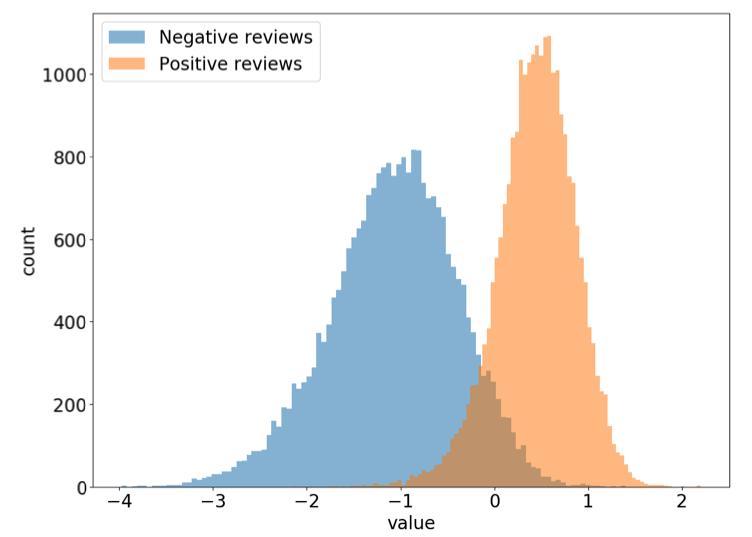
\includegraphics[height=3cm]{figures/sentiment}
        \caption{\href{https://arxiv.org/abs/1704.01444}{Sentiment neuron} [Radford et al., 2017]}
    \end{figure}
\end{frame}

\begin{frame}
    {Representation learning}
    What can we do with good representations:\\
    \begin{itemize}
        \item Learning with small data: fine-tuning on learned representations
        \item Transfer learning: one representation for many tasks 
        \item Metric learning: get a similarity metric for free 
    \end{itemize}

    \pause
    Training a neural network on any task gives us a representation good for \textit{that task}.

    But on which task can we learn good \textit{general} representations?
    %\begin{itemize}
    %    \item \textbf{}Self-supervised learning: obtain representations through generative modeling
    %\end{itemize}
\end{frame}

\begin{frame}
    {What can we learn from word guessing?}
    \begin{itemize}
        \itemsep1em
        \item The cats that are raised by my sister \rule{1.5cm}{0.5mm} sleeping. \pause\hfill \textit{syntax}
        \item Jane is happy that John invited \rule{1.5cm}{0.5mm} friends to his birthday party. \pause\hfill \textit{coreference}
        \item \rule{1.5cm}{0.5mm} is the capital of Tanzania. \pause\hfill \textit{knowledge}
        \item The boy is \rule{1.5cm}{0.5mm} because he lost his keys.  \pause\hfill \textit{coonsense}
        \item John took 100 bucks to Vegas. He won 50 and then lost 100. Now he only has \rule{1.5cm}{0.5mm} to go home. \pause\hfill \textit{nuerical reasoning}
    \end{itemize}

    \pause\bigskip
    Word guessing entails lots of tasks related to language understanding!
\end{frame}

\begin{frame}
    {Self-supervised learning}

    \textbf{Key idea}: predict parts of the input from the rest\\
    \begin{itemize}
        \item \blue{No supervision} is needed---both input and output are from the raw data.
        \item Easy to \blue{scale}---only need unlabeled data.
        \item Learned representation is \blue{general}---related to many tasks.
    \end{itemize}

    \pause
    \textbf{Approach}:\\
    \begin{itemize}
        \item \textbf{Pretrain}: train a model using self-supervised learning objectives on large data.
        \item \textbf{Finetune}: update part or all of the parameters of the pretrained model (which provides an initialization) on supervise data of a task.
    \end{itemize}
\end{frame}

\begin{frame}
    {A bit of history}
    \begin{itemize}[<+->]
        \item Pretrain an \blue{RNN} model on unlabeled data and finetune on supervised tasks
            \href{https://arxiv.org/pdf/1511.01432.pdf}{[Dai et al., 2015]}
            \href{https://arxiv.org/pdf/1511.01432.pdf}{[ULMFiT; Howard et al., 2018]}
            \begin{itemize}[<.->]
                \item Promising results on a small scale
            \end{itemize}
        \item ELMo: replace static word embedding by \blue{contextual word embeddings} from pretrained bi-LSTM \href{https://arxiv.org/abs/1802.05365}{[Peters et al., 2018]}
            \begin{itemize}[<.->]
                \item First impactful result in NLP
            \end{itemize}
        \item Pretrain a \blue{Transformer} model and finetune on supervised tasks 
            \begin{itemize}[<.->]
                \item GPT \href{https://s3-us-west-2.amazonaws.com/openai-assets/research-covers/language-unsupervised/language_understanding_paper.pdf}{[Radford et al., 2018]},
                    BERT \href{https://arxiv.org/abs/1810.04805}{[Devlin et al., 2018]}
            \end{itemize}
        \item \blue{Scale} the pretrained model to larger sizes
            \begin{itemize}[<.->]
                \item GPT-2 (1.5B), T5 (11B), GPT-3 (175B), PaLM (540B) 
                \item We will talk about 100B+ models in the third module
            \end{itemize}
    \end{itemize}
\end{frame}

\begin{frame}
    {Types of pretrained models}
   
    \begin{itemize}[<+->]
        \itemsep1em
        \item \textbf{Encoder models}, e.g., BERT
            \begin{itemize}[<.->]
                \item Encode text into vector representations that can be used for downstream classification tasks
            \end{itemize}
        \item \textbf{Encoder-decoder models}, e.g., T5
            \begin{itemize}[<.->]
                \item Encode input text into vector representations and generate text conditioned on the input
            \end{itemize}
        \item \textbf{Decoder models}, e.g., GPT-2 (later)
            \begin{itemize}[<.->]
                \item Read in text (prefix) and continue to generate text
            \end{itemize}
    \end{itemize}

    \pause\medskip
    All models are transformer based.
\end{frame}

\begin{frame}
    {Encoder models}
    
    An encoder takes a sequence of tokens and output their contextualized representations:
    $$
        h_1,\ldots,h_n = \mathrm{Encoder}(x_1,\ldots,x_n)
    $$
    We can then use $h_1,\ldots,h_n$ for other tasks.

    \pause\bigskip
    How do we train $\mathrm{Encoder}$?\\
    \begin{itemize}
        \item Use any supervised task: $y=f(h_1,\ldots,h_n)$
        \item Use self-supervised learning: predict a word from its neighbors 
    \end{itemize}
\end{frame}

\begin{frame}
    {Masked language modeling}

    Learning objective:\\
    $$
    \max \sum_{x\in\sD, i\sim p_{\text{mask}}} \log p(x_i\mid x_{-i}; \theta)
    $$
    \vspace{-1em}
    \begin{itemize}
        \item $x_{-i}$: noisy version fo $x$ where $x_i$ is corrupted
        \item $p_{\text{mask}}$: mask generator
    \end{itemize}

    \vspace{3.5cm}
\end{frame}

\begin{frame}
    {BERT: objective}

        \begin{itemize}
            \item \textbf{Masked language modeling}:
                \begin{itemize}
                    \item Randomly sample 15\% tokens as prediction targets
                    \item Replace the target tokens in the input by either \texttt{[MASK]} (10\%) or a random token (10\%), or leave it unchanged\\
                        cats \blue{are} cute $\rightarrow$
                        cats \blue{\texttt{[MASK]}/is/are} cute
                        
                    \item Later work has shown that just use \texttt{[MASK]} is sufficient
                \end{itemize}
            \pause
            \item \textbf{Next sentence prediction}: predict whether a pair of sentences are consecutive
                $$
                \max \sum_{x\sim\sD, x_{n}\sim p_{\text{next}}} \log p(y\mid x, x_n; \theta)
                $$
                \vspace{-1em}
                \begin{itemize}
                    \item $x_n$: either the sentence following $x$ or a randomly sampled sentence
                    \item $y$: binary label of whether $x_n$ follows $x$
                    \item Later work has shown that this objective is not necessary 
                \end{itemize}
        \end{itemize}
\end{frame}

\begin{frame}
    {BERT: architecture}
    \begin{figure}
            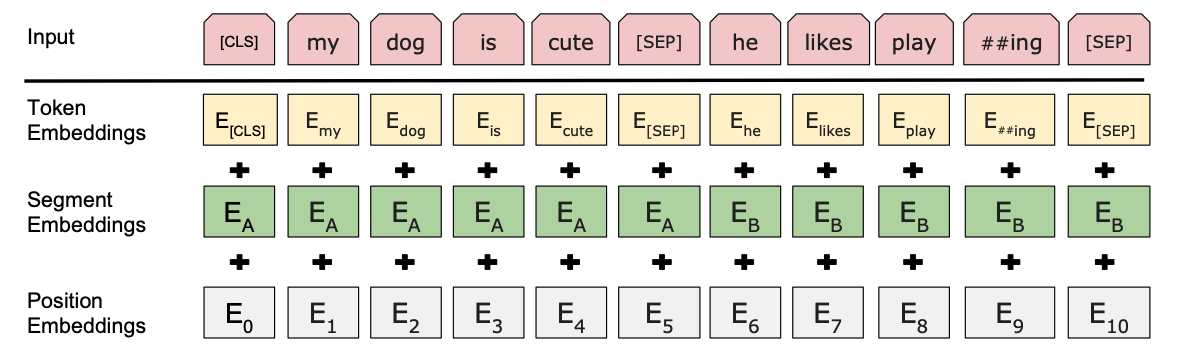
\includegraphics[width=.9\textwidth]{figures/bert}
    \end{figure}
    \vspace{-1em}
    \begin{itemize}[<+->]
        \item Subword unit: wordpiece (basically byte pair encoding) 
        \item \texttt{[CLS]}: first token of all sequences; used for next sentence prediction
        \item Distinguish two sentences in a pair: \texttt{[SEP]} and segment embedding
        \item Learned position embedding
        \item 12 (base; 110M params) or 24 (large; 340M params) layer Transformer
    \end{itemize}
\end{frame}

\begin{frame}
    {Finetuning BERT}
        Classification tasks:
            Add a linear layer (randomly initialized) on top of the \texttt{[CLS]} embedding
            $$
            p(y\mid x) = \mathrm{softmax}(Wh_{\text{[CLS]}})
            $$
            \begin{figure}
                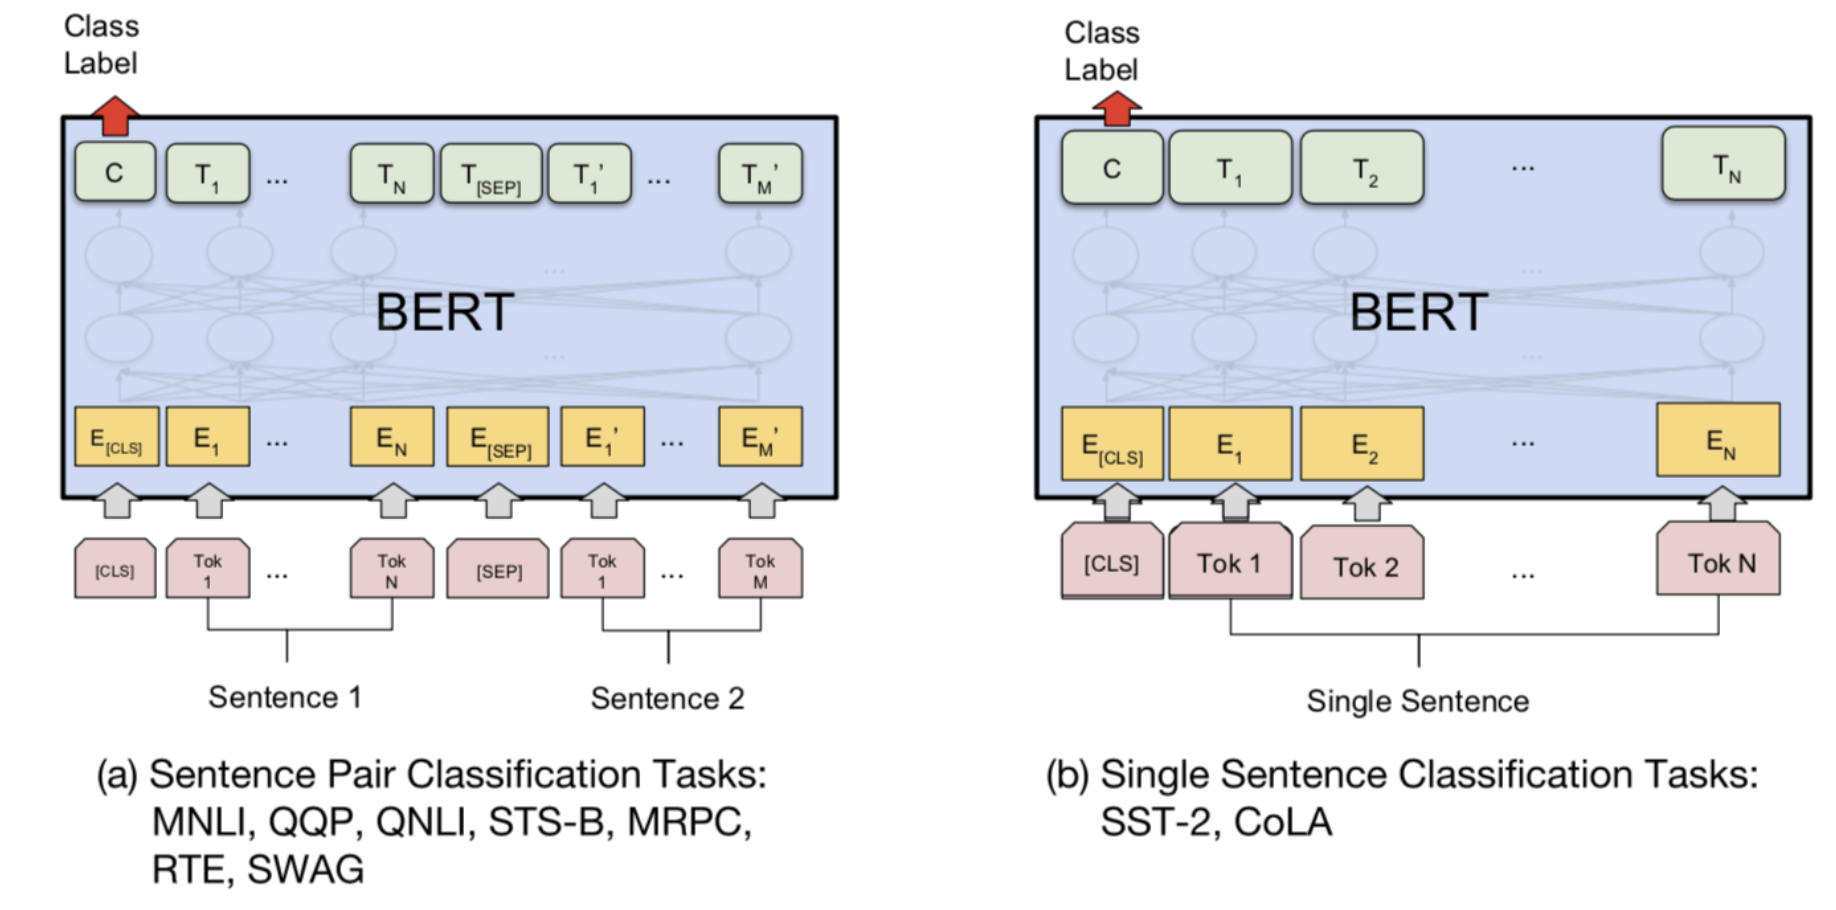
\includegraphics[width=0.8\textwidth]{figures/bert-classification}
            \end{figure}
\end{frame}

\begin{frame}
    {Finetuning BERT}
        Sequence labeling tasks:
            Add linear layers (randomly initialized) on top of every token 
            $$
            p(y_i \mid x) = \mathrm{softmax}(Wh_{i})
            $$
            \begin{figure}
                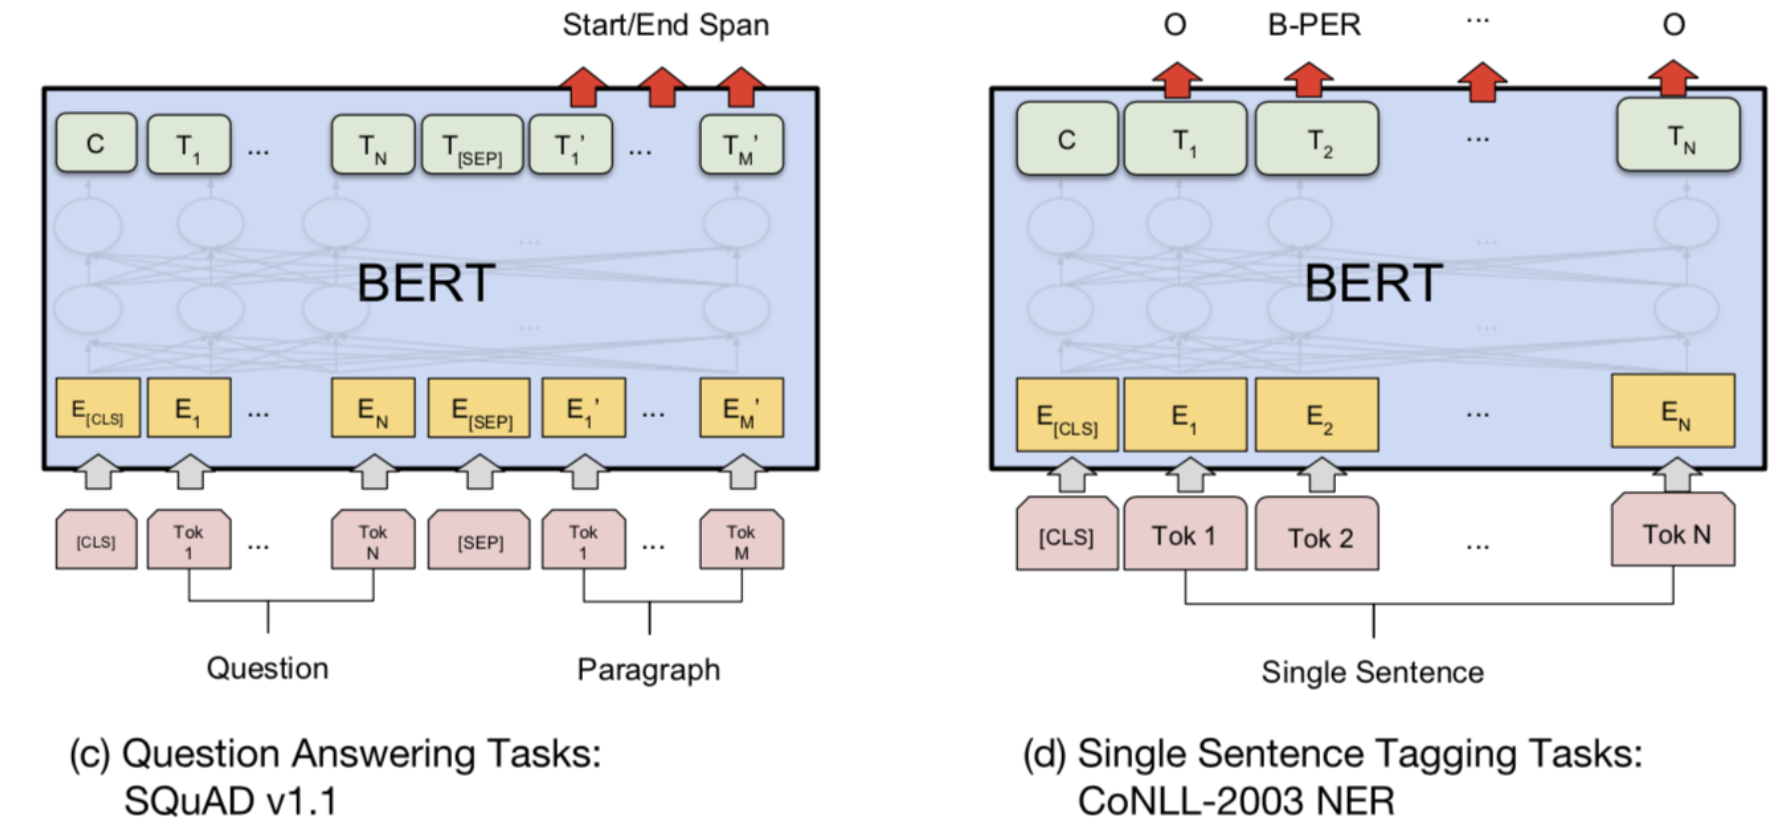
\includegraphics[width=0.8\textwidth]{figures/bert-seq-label}
            \end{figure}
\end{frame}

\begin{frame}
    {Finetuning BERT}

    \begin{itemize}
        \item Finetune all parameters (both the newly added layer and the pretrained weights)
        \item Use a small learning rate (e.g., 1e-5)
        \item Train for a small number of epochs (e.g, 3 epochs)
        \item Led to SOTA results on many NLU tasks
        \item Not straightforward to use on text generation tasks
    \end{itemize}
\end{frame}

\begin{frame}
    {Encoder-decoder models}

    An encoder-decoder model encodes input text to a sequence of contextualized representations, and decodes a sequence of tokens autoregressively.
    \begin{align*}
        h_1,\ldots,h_n &= \mathrm{Encoder}(x_1,\ldots,x_n) \\
        s_1,\ldots,s_m &= \mathrm{Decoder}(y_0,\ldots,y_{m-1}, h_1,\ldots,h_n)\\
        p(y_i\mid x, y_{<i}) &= \mathrm{softmax}(Ws_i)
    \end{align*}

    How do we train the encoder-decoder?
    \begin{itemize}
        \item Use any supervised task, e.g., machine translation 
        \item Use self-supervised learning: predict text spans from their neighbors 
    \end{itemize}
\end{frame}

\begin{frame}
    {Masked language modeling using an encoder-decoder}

    \textbf{Input}: text with corrupted spans\\
    \textbf{Output}: recovered spans

    \begin{figure}
        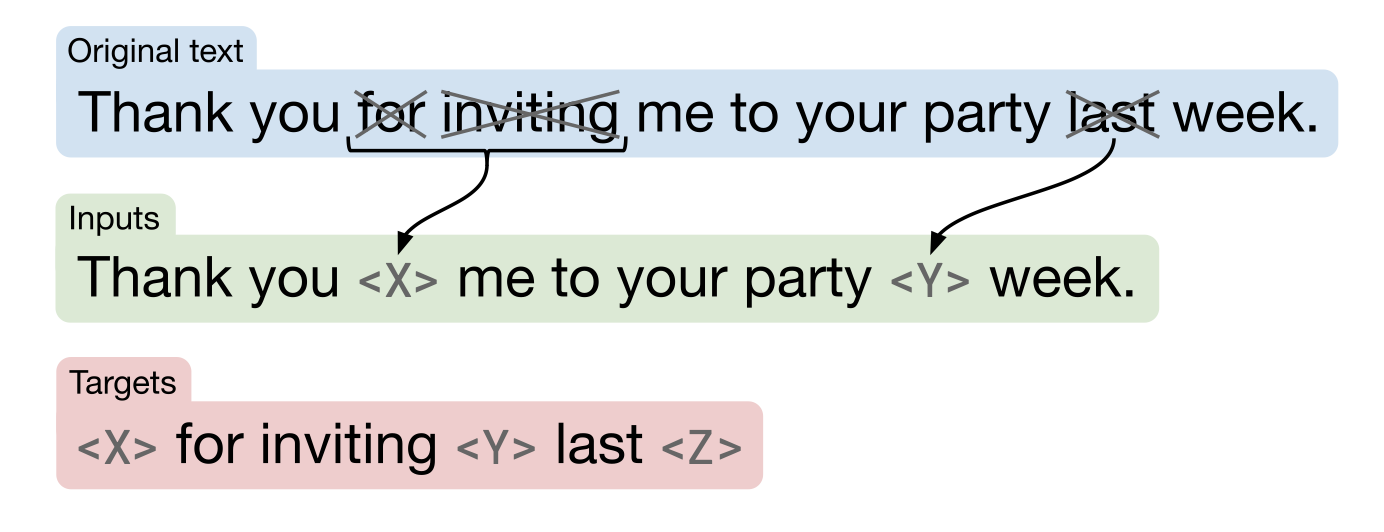
\includegraphics[height=3cm]{figures/t5-span}
    \end{figure}
\end{frame}

\begin{frame}
    {T5}

    \begin{itemize}
        \item First train on unlabele data by \textbf{masked language modeling}
            \begin{itemize}
                \item Predict corrupted spans as a sequence
            \end{itemize}
        \item Then continue training by \textbf{supervised multitask learning}
            \begin{itemize}
                \item Formulate tasks as text-to-text format
                \item Use a prefix to denote the task
                \item Mixing examples from different datasets when constructing batches  
            \end{itemize}
    \begin{figure}
        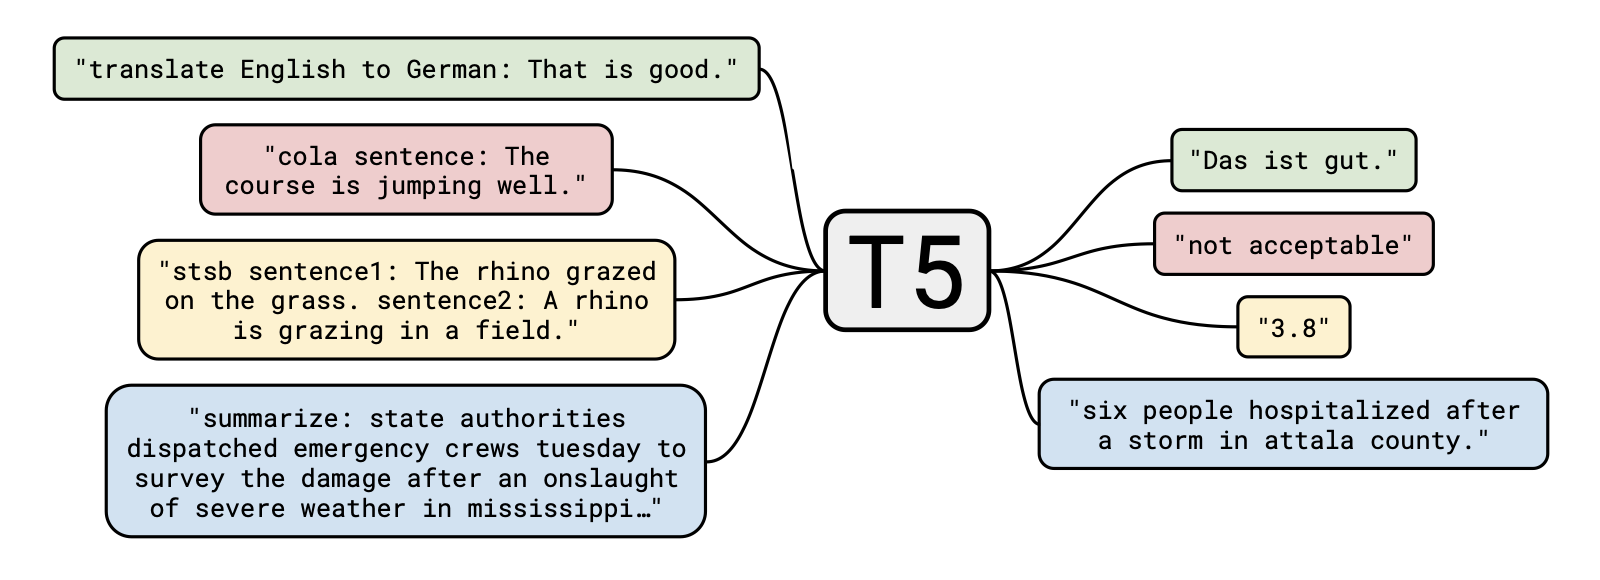
\includegraphics[height=4cm]{figures/t5-mtl}
    \end{figure}
        \item Jointly training with the two objectives works slightly worse
    \end{itemize}
\end{frame}

\begin{frame}
    {Finetuning T5}
    \begin{itemize}
        \item Formulate the task in text-to-text format
        \item Fine-tune all parameters (similar to BERT fine-tuning)
        \item Advantages over encoder models: unified modeling of many different tasks 
    \end{itemize}
\end{frame}

\begin{frame}
    {Efficient pretraining}

    An obvious downside of pretrained models is that they are quite expensive to train!

    How can we make them more efficient?\pause

    Idea 1: reducing the number of parameters smartly

    Example: ALBERT (a lite BERT) [Lan et al., 2020]

    \begin{itemize}
            \only<1>{
        \item \textbf{Factorization}:
    \begin{itemize}
        \item Recall that in Transformer, we first need to map the one-hot encoding (of size $\red{V}$) of a token to Q, K, V embeddings (of size $\blue{H}$)
        \item The number of parameters is $\red{V}\times \blue{H}$
        \item We can instead first map it to a lower-dim space (of size $\green{E}$) so that the number of params is $\red{V}\times\green{E} + \green{E}\times\blue{H}$
    \end{itemize}
}
            \only<2->{
\item \textbf{Parameter sharing}:
    \begin{itemize}
        \item Share feedforward network weights across layers
        \item Share self-attention weights across layers
        \item ALBERT: share all params across layers
    \end{itemize}
}
    \end{itemize}
\end{frame}

\begin{frame}
    {Efficient pretraining}
    Idea 2: design harder learning objectives

    ALBERT: Inter-sentence coherence loss\\
    \begin{itemize}
        \item Motivation: the next sentence prediction task is too easy
        \item Design \blue{hard negative examples}
        \item Input: take two consecutive sentences, swap their order randomly
        \item Output: predict if they are in natural order\\
            \begin{tabular}{ll}
                \textit{I went home. \texttt{SEP} I slept.} & +1\\
                \textit{I slept. \texttt{SEP} I went home.} & -1\\
            \end{tabular}
            
        \item What is needed to perform this task well?
    \end{itemize}
\end{frame}

\begin{frame}
    {Efficient pretraining}
    Idea 2: design harder learning objectives

    ELECTRA [Clark et al., 2020]: discriminate from true vs guessed tokens

    \vspace{-1em}
    \begin{figure}
        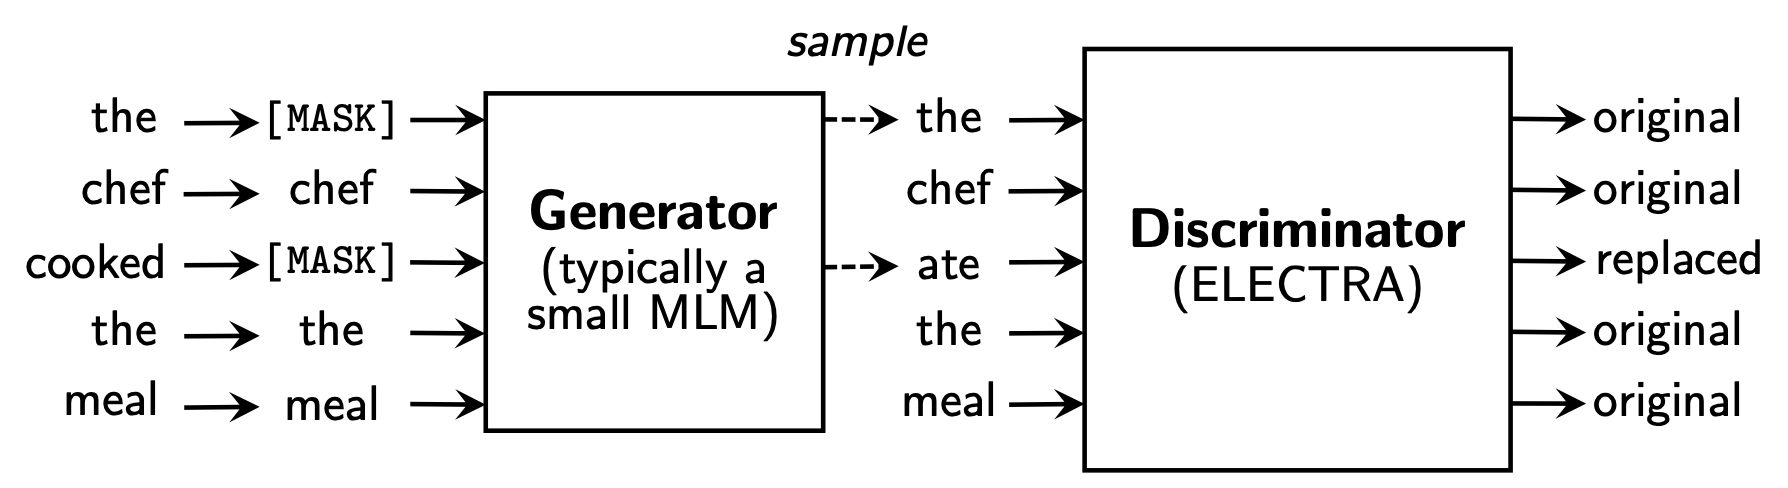
\includegraphics[height=3cm]{figures/electra}
    \end{figure}
    \vspace{-1em}

    \begin{itemize}
        \item First train the generator for n steps using the MLM objective.
        \item Freeze generator weights. Then train the discriminator using the sequence classification objective.
        \item The discriminator and generator share weights except for the input token embeddings.
    \end{itemize}
\end{frame}

\begin{frame}
    {Efficient pretraining}
    ELECTRA result:
    \begin{figure}
        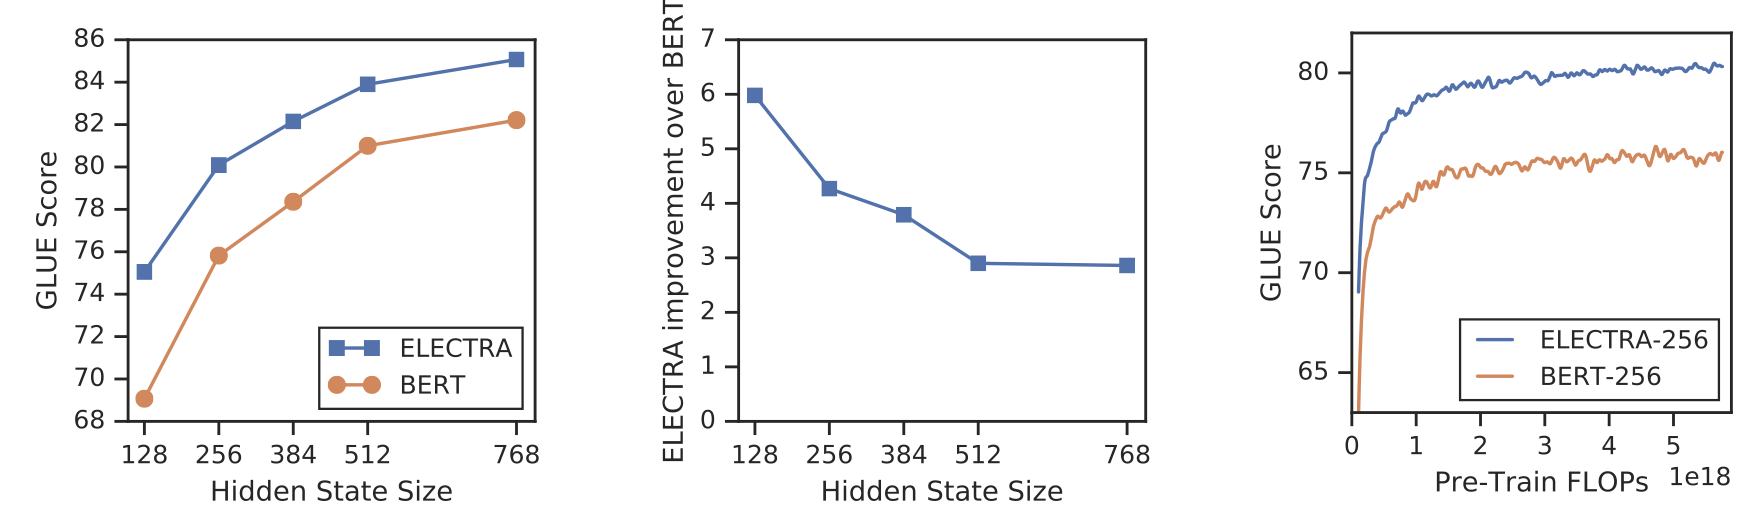
\includegraphics[height=3cm]{figures/electra-result}
        \caption{Finetuning result on the GLUE benchmark}
    \end{figure}
    \begin{itemize}
        \item Larger improvement at smaller model sizes
        \item Faster training 
        \item An effective approach if you don't have large compute for pretraining
    \end{itemize}
\end{frame}

\begin{frame}
    {What are these models trained on?}

    Both quantity and quality are important
    \begin{itemize}
        \item Wikipedia: encyclopedia articles (\green{clean}, \red{single domain})
        \item Toronto Books Corpus: e-books (\green{diverse domain}) 
        \item WebText (40GB): content submitted to Reddit with a vote $\ge 3$ (\green{diverse}, \red{bias}) 
        \item CommonCrawl (20TB): scraped HTML with markers removed (\green{diverse, large}, \red{noisy, bias})
            \begin{itemize}
                \item A cleaned version: C4 (750GB)
            \end{itemize}
    \end{itemize}
\end{frame}

\begin{frame}
    {Summary}

    Lots of learning happens from just observing the world (data).
    \begin{itemize}
        \item Self-supervised learning: \blue{benefits from large data and compute}
            \begin{itemize}
                \item Basic: predict parts from other parts based on the structure of data (works beyond text)
                \item Advanced: design hard negatives to improve efficiency
            \end{itemize}
        \item Finetuning: adapt pretrained models to downstream tasks on a small amount of labeled data
    \end{itemize}
\end{frame}


\end{document}
